The work offered several implementations of Machine Learning algorithms for State of Charge Estimation over A123 batteries.
The computation of the accuracies, recently summarised in \mbox{Tables~\ref{tab:acc-results1} and~\ref{tab:acc-results2}}, has involved multi-device calculations.
The measurement has been performed over the entire dataset of each profile.
Therefore, a synchronisation strategy has been attempted to speed up the process and keep devices temperature safe.
Fans at 45-50\% duty cycle kept temperatures within 45-52 degrees range.
A small timeout to switch between sample intensive datasets allowed GPUs to cool off between models.
%
% IF
\ifthenelse {\boolean{thesis}}
%
% THEN
{
\mbox{Figure~\ref{fig:device_compute}} demonstrates the paralysation mechanism for a single model, where flops and the total number of parameters are determined using the script in Appendix~\ref{app:flops}.
}
{
\mbox{Figure~\ref{fig:device_compute}} demonstrates the paralysation mechanism for a single model.
}
Since the CPU has the lowest compute rating, it attempted only a single dataset, while 2 GPUs handled between 6-8 sets together. 

%
%
Since the end goal is to deploy an electric vehicle to run processing online, there have been several attempts to measure performance on a few categories of embedded devices.
By itself, Stateful models are not supported by TFLite.
Thus, a single attempt to make a Custom Stateful stateless model test is time inefficient, and those seemed unreasonable.
Instead, six models were broke down into five foundation implementations and performance profiled, \mbox{Table~\ref{tab:speed}}.
Calculation of accuracies performed with 20 attempts average and offset calculation with mean of the difference between maximum and minimum.
As a result, Coral TPU has an advantage over Raspberrypi since the core is dedicated to run tensor computations, despite Pi's latest hardware release.
The android selection only proved how time-consuming usage of ML model on relatively old CPU could be, but in a proper synchronised manner and without rapid consumption, such devices still have their usage in such application.
% Steady Voltage consumption over USB Port stable around 5.03V for all devices. Coral TPU steady current - 0.07A. Keep those details for the Ch5 if asked.
\textcolor{red}{\textbf{When Testing validation process  with plot generation was performen on TPU deices using TFLite, the accuracy degradation and overall accuracy against entire dataset was calculated using GPUs and CPU.}}
\begin{figure}[ht]
    \centering
    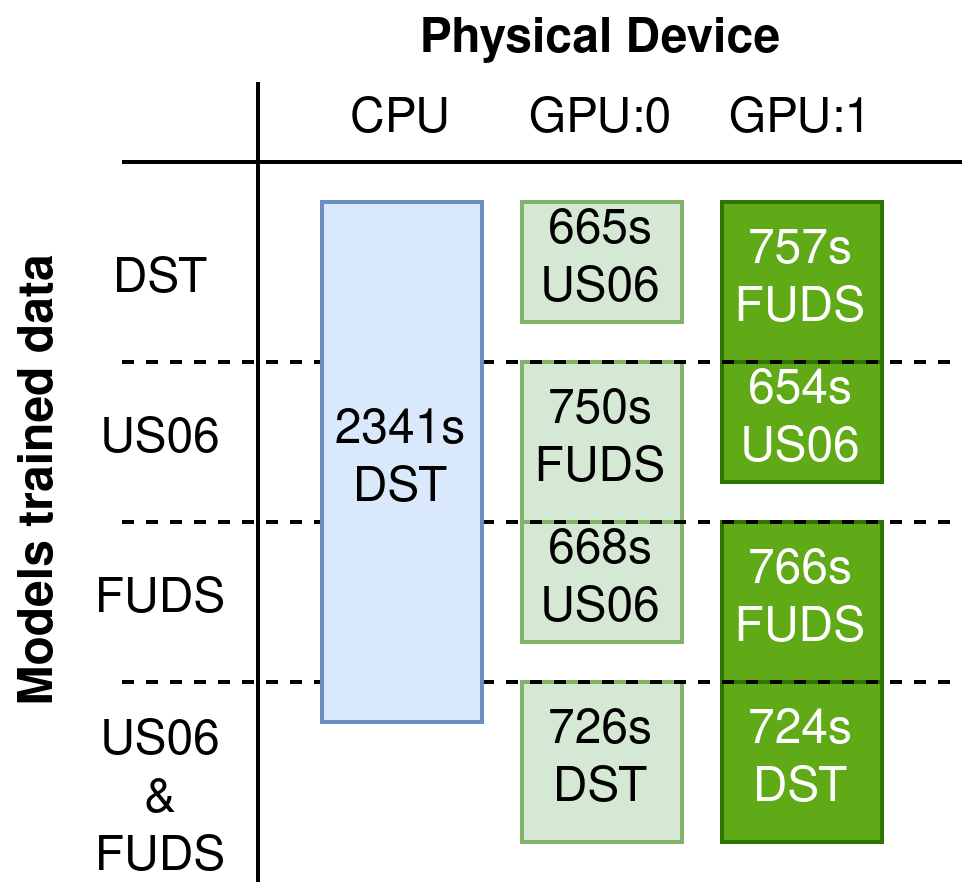
\includegraphics[width=\columnwidth]{II_Body/images/Accuracy_Compute.png}
    % \includesvg[width=\linewidth]{II_Body/images/Accuracy_Compute_10.svg}
    \caption{Accuracy computation using a single model trained on different proflies separately. The timing examples were taken from Model \#5 computation process.}
    \label{fig:device_compute}
\end{figure}
\begin{table*}[ht]
    \renewcommand{\arraystretch}{1.3}
    \caption{Model performance results across multiple embedded devices.}
    \centering
    \label{tab:speed}
    \resizebox{\linewidth}{!}{
    \begin{tabular}{l c c |c c c}
        \hline\hline \\[-4mm]
        Structure                &Total params& flop/it & Coral TPU (ms) & R-Pi4 (ms)      & Android (ms) \\
        \hline
        1 $\times$ LSTM(500)     & 1,008,501  & 2.0G & 227.9$\pm$17.2 & 2021.6$\pm$164.9 & 4058.7$\pm$45.0 \\% 4048.0$\pm$69.0 \\   %FLOPs:2,018,005
        1 $\times$ GRU(560)      & 949,761    & 1.9G & 198.3$\pm$36.6 & 2104.2$\pm$109.6 & 3809.2$\pm$41.5 \\%3815.9$\pm$33.0 \\   %FLOPs:189,903
        LSTM(500) \& Atten
                                 & 1,361,881  & 3.2G & 206.9$\pm$32.9 & 2125.2$\pm$126.1 & 4711.2$\pm$51.0 \\%4711.8$\pm$41.5 \\ %FLOPs:3,222,344
%        2 $\times$ GRU(60)       & 33,762     & Unkn & ** & ** & \\
        1 $\times$ GRU(500)      & 758,001    & 1.5G & 140.8$\pm$24.7 & 1816.1$\pm$129.1 & 3227.5$\pm$37.5 \\%3241.7$\pm$32.5 \\  % FLOPs:1,516,503
        2 $\times$ LSTM(250)     & 504,201    & 1.1G & 102.2$\pm$16.3 & 1802.6$\pm$131.1 & 2494.4$\pm$34.0 \\%2454.4$\pm$33.0 \\   % FLOPs:1,109,409
%        1 $\times$ Layer \& Dense& 3,369      &     & 2.35$\pm$0.25  & 3.15$\pm$0.85 & 6.3*\\
        \hline\hline
    \end{tabular}
    }
\end{table*}
